%%%%%%%%%%%%%%%%%%%%%%%%%%%%%%%%%%%%%%%%%%%%%%%%%%%%
%%%%%%%%%%% NU para la velocidad %%%%%%%%%%%%%%%%%%%
%%%%%%%%%%%%%%%%%%%%%%%%%%%%%%%%%%%%%%%%%%%%%%%%%%%%
\def\vNUa%
{
%% Dibuja una cajita!! %%%%%%%%%%%%%%%%%%%
%% el background de gris..
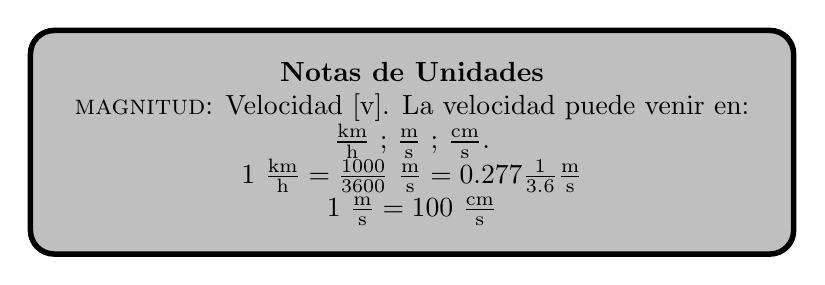
\begin{tikzpicture}
  \node[rectangle, rounded corners=0.3cm, 
  fill=lightgray, draw, line width=2pt, 
  inner sep=10pt] {
    \begin{tabular}{c}
%%%%%%%%%%%%%%%%%%%%%%%%%%%%%%%%%%%%%%%%%%
{\bf Notas de Unidades}\\
{\sc magnitud}: Velocidad [v].
La velocidad puede venir en: \\

$\frac{{\rm km}}{{\rm h}}$ ; 
$\frac{{\rm m}}{{\rm s}}$ ; 
$\frac{{\rm cm}}{{\rm s}}$. \\

$1~\frac{{\rm km}}{{\rm h}}=
\frac{1000}{3600}~\frac{{\rm m}}{{\rm s}}
=\cancelto{0.277}{\frac{1}{3.6}}\frac{{\rm m}}{{\rm s}}$ \\

$1~\frac{{\rm m}}{{\rm s}} = 100~\frac{{\rm cm}}{{\rm s}}$

%%%%%%%%%%%%%%%%%%%%%%%%%%%%%%%%%%%%%%%%%%
\end{tabular}
  };
\end{tikzpicture}
%%%%%%%%%%%%%%%%%%%%%%%%%%%%%%%%%%%%%%%%%%

%% fin definicion de vNUa
}
%%%%%%%%%%%%%%%%%%%%%%%%%%%%%%%%%%%%%%%%%%%%%%%%%%%%
%%%%%%%%%%%%%%%%%%%%%%%%%%%%%%%%%%%%%%%%%%%%%%%%%%%%
%%%%%%%%%%%%%%%%%%%%%%%%%%%%%%%%%%%%%%%%%%%%%%%%%%%%
